\section{Concavity and the Second Derivative}\label{sec:concavity}

Our study of ``nice'' functions continues. The previous section showed how the first derivative of a function, \fp, can relay important information about $f$. We now apply the same technique to \fp\ itself, and learn what this tells us about $f$.

The key to studying $\fp$ is to consider its derivative, namely  $\fp'$, which is the second derivative of $f$.  When $\fp'>0$, $\fp$ is increasing. When $\fp'<0$, \fp\ is decreasing.  $\fp$ has relative maxima and minima where $\fp'=0$ or is undefined.

This section explores how knowing information about \fpp\ gives information about $f$.\\ %reaches its maximum rate of increase or decrease, in other words, when the function is changing at its most rapid rate, we usually have $f''=0$.

\noindent\textbf{\large Concavity}
\vskip \baselineskip

We begin with a definition, then explore its meaning.

\definition{def:concavity}{Concave Up and Concave Down}%
{Let $f$ be differentiable on an interval $I$. 
The graph of $f$ is \textbf{concave up} on $I$ if $\fp$ is increasing. The graph of $f$ is \textbf{concave down} on $I$ if $\fp$ is decreasing. If $\fp$ is constant then the graph of $f$ is said to have \textbf{no concavity}.\index{concavity}\index{concave up}\index{concave down}
}

\mnote{.62}{\textbf{Note:} We often state that ``$f$ is concave up'' instead of ``the graph of $f$ is concave up'' for simplicity.}

The graph of a function $f$ is \textit{concave up} when \fp\ is \textit{increasing.} That means as one looks at a concave up graph from left to right, the slopes of the tangent lines will be increasing. Consider Figure \ref{fig:concavity1}, where a concave up graph is shown along with some tangent lines. Notice how the tangent line on the left is  steep, downward, corresponding to a  small value of \fp. On the right, the tangent line is steep, upward, corresponding to a large value of \fp.

\mfigure{.8}{A function $f$ with a concave up graph. Notice how the slopes of the tangent lines, when looking from left to right, are increasing.}{fig:concavity1}{figures/figconcavity1}
%
%When $f''>0$, the shape of the graph of $f$ looks like a part of the graph below.
%\begin{center}\myincludegraphics[scale=.3]{apex-second-derivative_img1}\end{center}
%The function is said to be \emph{concave up} when it looks like this.  
%  The second derivative is positive precisely where the function is concave up.

If a function is decreasing and concave up, then its rate of decrease is slowing; it is ``levelling off.''  If the  function is increasing and concave up, then the \textit{rate} of increase is increasing.  The function is increasing at a faster and faster rate.

Now consider a function which is concave down. We essentially repeat the above paragraphs with slight variation.

The graph of a function $f$ is \textit{concave down}  when \fp\ is \textit{decreasing.} That means as one looks at a concave down graph from left to right, the slopes of the tangent lines will be decreasing. Consider Figure \ref{fig:concavity2}, where a concave down graph is shown along with some tangent lines. Notice how the tangent line on the left is  steep, upward, corresponding to a large value of \fp. On the right, the tangent line is steep, downward, corresponding to a small value of \fp.%

\mfigure{.35}{A function $f$ with a concave down graph. Notice how the slopes of the tangent lines, when looking from left to right, are decreasing.}{fig:concavity2}{figures/figconcavity2}
\enlargethispage{\baselineskip}

If a function is increasing and concave down, then its rate of increase is slowing; it is ``levelling off.''  If the function is decreasing and concave down, then the \textit{rate} of decrease is decreasing.  The function is decreasing at a faster and faster rate.

\mnote{.55}{\textbf{Note:} A mnemonic for remembering what concave up/down means is: ``Concave up is like a cup; concave down is like a frown.'' It is admittedly terrible, but it works.
%
%A mnemonic for remembering how to pronounce ``mnemonic'' is to recall it begins with the same sound as ``mnemotechnic.''
} 

Our definition of concave up and concave down is given in terms of when the first derivative is increasing or decreasing. We can apply the results of the previous section and to find intervals on which a graph is concave up or down. That is, we recognize that $\fp$ is increasing when $\fpp>0$, etc. 

\theorem{thm:concavity}{Test for Concavity}%
{Let $f$ be twice differentiable on an interval $I$. The graph of $f$ is concave up if $\fpp>0$ on $I$, and is concave down if $\fpp<0$ on $I$. \index{concavity!test for}\index{concavity!inflection point}
}


%\paragraph{Concave down}
%When $f''<0$, the shape of the graph of $f$ looks like a part of the graph below.
%
%%\begin{center}\myincludegraphics[scale=.3]{apex-second-derivative_img2}\end{center}
%
%The function is said to be \emph{concave down} when it looks like this.  Geometrically, a function is concave down if its graph lies below all of its tangent lines. The second derivative is negative precisely where the function is concave down.
%
%If a function is increasing and concave down, then the rate of increase is slowing down and the function is leveling off.  On the other hand, if the function is decreasing and concave down, then it is decreasing at a faster and faster rate.

%\ifthenelse{\boolean{longpage}}{\vskip \baselineskip}{}

\mnote{.12}{\textbf{Note:} Geometrically speaking, a function is concave up if its graph lies above its tangent lines. A function is concave down if its graph lies below its tangent lines.}

If knowing where a graph is concave up/down is important, it makes sense that the places where the graph changes from one to the other is also important. This leads us to a definition.

\mfigure{.8}{Demonstrating the 4 ways that concavity interacts with increasing/decreasing, along with the relationships with the first and second derivatives.}{fig:concavity3}{figures/figconcavity3}

\definition{def:infl}{Point of Inflection}
{A \textbf{point of inflection} is a point on the graph of $f$ at which the concavity of $f$ changes.\index{point of inflection}\index{inflection point}
}

Figure \ref{fig:concavity4} shows a graph of a function with inflection points labelled.

\mfigure{.55}{A graph of a function with its inflection points marked. The intervals where concave up/down are also indicated.}{fig:concavity4}{figures/figconcavity4}

If the concavity of $f$ changes at a point $(c,f(c))$, then \fp\ is changing from increasing to decreasing (or, decreasing to increasing) at $x=c$. That means that the sign of \fpp\ is changing from positive to negative (or, negative to positive) at $x=c$.  This leads to the following theorem.

\theorem{thm:inflection}{Points of Inflection}
{If $(c,f(c))$ is a point of inflection on the graph of $f$, then either $\fpp(c)=0$ or $\fpp$ is not defined at $c$.}

We have identified the concepts of concavity and points of inflection. It is now time to practice using these concepts; given a function, we should be able to find its points of inflection and identify intervals on which it is concave up or down. We do so in the following examples.\\


%\myincludegraphics[scale=.5]{apex-second-derivative_img3} % function for this image is $x^5-3x^3+2x+1$

\example{ex_conc1}{Finding intervals of concave up/down, inflection points}{
Let $f(x)=x^3-3x+1$. Find the inflection points of $f$ and the intervals on which it is concave up/down.}
{We start by finding $\fp(x)=3x^2-3$ and $\fpp(x)=6x$.  To find the inflection points, we use Theorem \ref{thm:inflection} and find where $\fpp(x)=0$ or where \fpp\ is undefined. We find \fpp\ is always defined, and is 0 only when $x=0$. So the point $(0,1)$ is the only possible point of inflection.

This possible inflection point divides the real line into two intervals, $(-\infty,0)$ and $(0,\infty)$. We use a process similar to the one used in the previous section to determine increasing/decreasing. Pick any $c<0$; $\fpp(c)<0$ so $f$ is concave down on $(-\infty,0)$. Pick any $c>0$; $\fpp(c)>0$ so $f$ is concave up on $(0,\infty)$. Since the concavity changes at $x=0$, the point $(0,1)$ is an inflection point.

The number line in Figure \ref{fig:concline1} illustrates the process of determining concavity; Figure \ref{fig:conc1} shows a graph of $f$ and \fpp, confirming our results. Notice how $f$ is concave down precisely when $\fpp(x)<0$ and concave up when $\fpp(x)>0$.
%\mfigure{.38}{A sign diagram for $\fpp$ determining the concavity of $f$ in Example \ref{ex_conc1}.}{fig:concline1}{figures/figconcline1}

\mtable{.38}{A sign diagram for $\fpp$ determining the concavity of $f$ in Example \ref{ex_conc1}.}{fig:concline1}{
\begin{center}
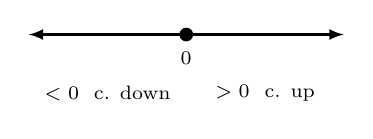
\begin{tikzpicture}[>=latex]
\draw [<->, thick] (-2,0) -- (2,0);
\draw [fill] (0,0) circle [radius=0.08];
\draw (0,-0.1) node[below] {\scriptsize \parbox{40pt}{\centering $0$}};
		
\draw (-1,-.75) node {\scriptsize \parbox{50pt}{\centering $\fpp<0$ \ c. down }};
\draw (1,-.75) node {\scriptsize \parbox{50pt}{\centering $\fpp>0$ \ c. up }};
\end{tikzpicture}
\end{center}}
%\myincludegraphics[scale=.5]{apex-second-derivative_img4}
\mfigure{.19}{A graph of $f(x)$ used in Example \ref{ex_conc1}.}{fig:conc1}{figures/figconc1}
}\\

\example{ex_conc2}{Finding intervals of concave up/down, inflection points}{
Let $f(x)=x/(x^2-1)$. Find the inflection points of $f$ and the intervals on which it is concave up/down.}
{We need to find \fp\ and \fpp. Using the Quotient Rule and simplifying, we find
\[
\fp(x)=\frac{-(1+x^2)}{(x^2-1)^2} \quad \text{and}\quad \fpp(x) = \frac{2x(x^2+3)}{(x^2-1)^3}.
\]

To find the possible points of inflection, we seek to find where $\fpp(x)=0$ and where $\fpp$ is not defined. Solving $\fpp(x)=0$ reduces to solving $2x(x^2+3)=0$; we find $x=0$.  We find that \fpp\ is not defined when $x=\pm 1$, for then the denominator of \fpp\ is 0. We also note that $f$ itself is not defined at $x=\pm1$, having a domain of $(-\infty,-1)\cup(-1,1)\cup(1,\infty)$. Since the domain of $f$ is the union of three intervals, it makes sense that the concavity of $f$ could switch across intervals. We technically cannot say that $f$ has a point of inflection at $x=\pm1$ as they are not part of the domain, but we must still consider these $x$-values to be important and will include them in our number line.

The important $x$-values at which concavity might switch are $x=-1$, $x=0$ and $x=1$, which  split the number line into four intervals as shown in Figure \ref{fig:concline2}. We determine the concavity on each. Keep in mind that all we are concerned with is the \textit{sign} of \fpp\ on the interval.\\

\noindent\textbf{Interval 1,} $(-\infty,-1)$: Select a number $c$ in this interval with a large magnitude (for instance, $c=-100$). The denominator of $\fp'(x)$ will be positive. In the numerator, the $(c^2+3)$ will be positive and the $2c$ term will be negative. Thus the numerator is negative and $\fpp(c)$ is negative. We conclude $f$ is concave down on $(-\infty,-1)$.

\noindent\textbf{Interval 2,} $(-1,0)$: For any number $c$ in this interval, the term $2c$ in the numerator will be negative, the term $(c^2+3)$ in the numerator will be positive, and the term $(c^2-1)^3$ in the denominator will be negative. Thus $\fpp(c)>0$ and $f$ is concave up on this interval.

\noindent\textbf{Interval 3,} $(0,1)$: Any number $c$ in this interval will be positive and ``small.'' Thus the numerator is positive while the denominator is negative. Thus $\fpp(c)<0$ and $f$ is concave down on this interval.

\noindent\textbf{Interval 4,} $(1,\infty)$: Choose a large value for $c$. It is evident that $\fpp(c)>0$, so we conclude that $f$ is concave up on $(1,\infty)$.


\noindent\begin{minipage}{\textwidth}\centering
%\myincludegraphics{figures/figconcline2}
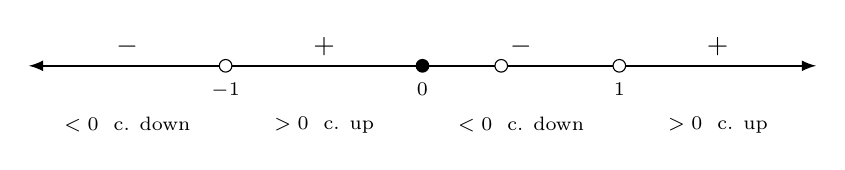
\begin{tikzpicture}[>=latex]

\draw [<->, thick] (-5,0) -- (5,0);
\foreach \x / \y  in %
					{%
					-2.5/{$-1$},%
					2.5/{$1$},%
					}
		{\draw [fill=white] (\x,0) circle [radius=0.08];
		 \draw (\x,-0.1) node[below] {\scriptsize \parbox{40pt}{\centering \y}};}

\draw [fill] (0,0) circle [radius=0.08];
		 \draw (0,-0.1) node[below] {\scriptsize \parbox{40pt}{\centering $0$}};
\draw (-3.75,-.75) node {\scriptsize \parbox{50pt}{\centering $\fpp<0$ \ c. down }};
\draw (-3.75,.25) node {$-$};
\draw (-1.25,-.75) node {\scriptsize \parbox{50pt}{\centering $\fpp>0$ \ c. up }};
\draw (-1.25,.25) node {$+$};
\draw (1.25,-.75) node {\scriptsize \parbox{50pt}{\centering $\fpp<0$ \ c. down }};
\draw (1.25,.25) node {$-$};
\draw (3.75,-.75) node {\scriptsize \parbox{50pt}{\centering $\fpp>0$ \ c. up}};
\draw (3.75,.25) node {$+$};

\end{tikzpicture}
\captionsetup{type=figure}%
\caption{Sign diagram for $\fpp$ in Example \ref{ex_conc2}.}\label{fig:concline2}
\end{minipage}\\

We conclude that $f$ is concave up on $(-1,0)\cup(1,\infty)$ and concave down on $(-\infty,-1)\cup(0,1)$. There is only one point of inflection, $(0,0)$, as $f$ is not defined at $x=\pm 1$. Our work is confirmed by the graph of $f$ in Figure \ref{fig:conc2}. Notice how $f$ is concave up whenever \fpp\ is positive, and concave down when \fpp\ is negative.
\mfigure{.8}{A graph of $f(x)$ and $\fpp(x)$ in Example \ref{ex_conc2}.}{fig:conc2}{figures/figconc2}
%\myincludegraphics[scale=.7]{apex-second-derivative_img5}
}\\
%\myincludegraphics[scale=.5]{apex-second-derivative_img6}

Recall that relative maxima and minima of $f$ are found at critical points of $f$; that is, they are found when $\fp(x)=0$ or when $\fp$ is undefined. Likewise, the relative maxima and minima of \fp\ are found when $\fpp(x)=0$ or when \fpp\ is undefined; note that these are the inflection points of $f$. 

What does a ``relative maximum of \fp\ '' \textit{mean}? The derivative measures the rate of change of $f$; maximizing \fp\ means finding  where $f$ is increasing the most -- where $f$ has the steepest tangent line. A similar statement can be made for minimizing \fp; it corresponds to where $f$ has the steepest negatively--sloped tangent line.

We utilize this concept in the next example.\\

\enlargethispage{\baselineskip}

\example{ex_conc3}{Understanding inflection points}{
The sales of a certain product over a three-year span are modelled by $S(t)= t^4-8t^2+20$, where $t$ is the time in years, shown in Figure \ref{fig:conc3}.  Over the first two years, sales are decreasing.  Find the point at which sales are decreasing at their greatest rate.

\mfigure{.2}{A graph of $S(t)$ in Example \ref{ex_conc3}, modelling the sale of a product over time.}{fig:conc3}{figures/figconc3}
}
{We want to maximize the rate of decrease, which is to say, we want to find where $S\primeskip'$ has a minimum.  To do this, we find where $S\primeskip''$ is 0.  We find $S\primeskip'(t)=4t^3-16t$ and $S\primeskip''(t)=12t^2-16$.  Setting $S\primeskip''(t)=0$ and solving, we get $t=\sqrt{4/3}\approx 1.16$ (we ignore the negative value of $t$ since it does not lie in the domain of our function $S$).

This is both the inflection point and the point of maximum decrease.  This is the point at which things first start looking up for the company.  After the inflection point, it will still take some time before sales start to increase, but at least sales are not decreasing quite as quickly as they had been.

A graph of $S(t)$ and $S\primeskip'(t)$ is given in Figure \ref{fig:conc3b}. When $S\primeskip'(t)<0$, sales are decreasing; note how at $t\approx 1.16$, $S\primeskip'(t)$ is minimized. That is, sales are decreasing at the fastest rate at $t\approx 1.16$.  On the interval of $(1.16,2)$, $S$ is decreasing but concave up, so the decline in sales is ``levelling off.''
}\\


%\myincludegraphics[scale=.5]{apex-second-derivative_img8}

Not every critical point corresponds to a relative extrema; $f(x)=x^3$ has a critical point at $(0,0)$ but no relative maximum or minimum. Likewise, just because $\fpp(x)=0$ we cannot conclude concavity changes at that point. We were careful before to use terminology ``\textit{possible} point of inflection'' since we needed to check to see if the concavity changed. The canonical example of $\fpp(x)=0$ \textit{without} concavity changing is $f(x)=x^4$. At $x=0$, $\fpp(x)=0$ but $f$ is always concave up, as shown in Figure \ref{fig:concavity5}.\\

\mfigure{.8}{A graph of $S(t)$ in Example \ref{ex_conc3} along with $S\primeskip'(t)$.}{fig:conc3b}{figures/figconc3b}

\mfigure{.55}{A graph of $f(x) = x^4$. Clearly $f$ is always concave up, despite the fact that $\fpp(x) = 0$ when $x=0$. It this example, the \textit{possible} point of inflection $(0,0)$ is not a point of inflection.}{fig:concavity5}{figures/figconcavity5}

%\paragraph{A note about concavity}
%
%In general, concavity can change only where either the second derivative is 0, where there is a vertical asymptote, or (rare in practice) where the second derivative is undefined.  But concavity doesn't \emph{have} to change at these places.  For instance, if $f(x)=x^4$, then $f''(0)=0$, but there is no change of concavity at 0 and also no inflection point there.   Moreover, if $f(x)=1/x^2$, then $f$ has a vertical asymptote at 0, but there is no change in concavity at 0.  See the figure below.

%\myincludegraphics[scale=.5]{apex-second-derivative_img7}


\noindent\textbf{\large The Second Derivative Test}
\vskip\baselineskip

The first derivative of a function gave us a test to find if a critical value corresponded to a relative maximum, minimum, or neither. The second derivative gives us another way to test if a critical point is a local maximum or minimum. The following theorem officially states something that is intuitive: if a critical value occurs in a region where a function $f$ is concave up, then that critical value must correspond to a relative minimum of $f$, etc. See Figure \ref{fig:concavity6} for a visualization of this.

\mfigure{.3}{Demonstrating the fact that relative maxima occur when the graph is concave down and relative minima occur when the graph is concave up.}{fig:concavity6}{figures/figconcavity6}

\theorem{thm:second_der}{The Second Derivative Test}%
{ Let $c$ be a critical value of $f$ where  $\fpp(c)$ is defined. \index{derivative!Second Deriv. Test}\index{Second Derivative Test}\index{extrema!and Second Deriv. Test}\index{maximum!and Second Deriv. Test}\index{minimum!and First Deriv. Test}
\begin{enumerate}
\item If $\fpp(c)>0$, then $f$ has a local minimum at $(c,f(c))$.
\item If $\fpp(c)<0$, then $f$ has a local maximum at $(c,f(c))$.
\end{enumerate}
}



%\myincludegraphics[scale=.7]{apex-second-derivative_img9}

The Second Derivative Test relates to the First Derivative Test in the following way. If $\fpp(c)>0$, then the graph is concave up at a critical point $c$ and $\fp$ itself is growing.  Since $\fp(c)=0$ and $\fp$ is growing at $c$, then it must go from negative to positive at $c$.  This means the function goes from decreasing to increasing, indicating a local minimum at $c$.\\
%\clearpage

\example{ex_conc4}{Using the Second Derivative Test}{
Let $f(x)=100/x + x$.  Find the critical points of $f$ and use the Second Derivative Test to label them as relative maxima or minima.}
{We find $\fp(x)=-100/x^2+1$ and $\fpp(x) = 200/x^3.$  We set $\fp(x)=0$ and solve for $x$ to find the critical values (note that \fp\ is not defined at $x=0$, but neither is $f$ so this is not a critical value.) We find  the critical values are $x=\pm 10$.  Evaluating \fpp\ at $x=10$ gives $0.1>0$, so there is a local minimum at $x=10$.  Evaluating $\fpp(-10)=-0.1<0$, determining a relative maximum at  $x=-10$. These results are confirmed in Figure \ref{fig:conc4}.
}\\

\mfigure{.78}{A graph of $f(x)$ in Example \ref{ex_conc4}. The second derivative is evaluated at each critical point. When the graph is concave up, the critical point represents a local minimum; when the graph is concave down, the critical point represents a local maximum.}{fig:conc4}{figures/figconc4}

We have been learning how the first and second derivatives of a function relate information about the graph of that function. We have found intervals of increasing and decreasing, intervals where the graph is concave up and down, along with the locations of relative extrema and inflection points. In Chapter \ref{chapter:limits} we saw how limits explained asymptotic behaviour. In the next section we combine all of this information to produce accurate sketches of functions.
%\myincludegraphics[scale=.7]{apex-second-derivative_img10}


\printexercises{exercises/03_04_exercises}
